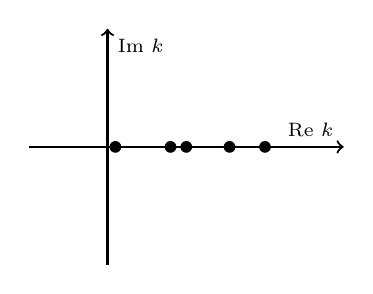
\begin{tikzpicture}
    \begin{scope}[thick,font=\scriptsize]
    % Axes:
    % Are simply drawn using line with the `->` option to make them arrows:
    % The main labels of the axes can be places using `node`s:

    %\draw [dashed] (-1.5,-3) -- (-1.5,3) {};

    %\draw node at (-1.5,-3.2) {$-\lambda_{*}$};

    %\fill[fill=black!20] (-3,-3) rectangle (-1.5,3);
    \draw [->] (-1,0) -- (3,0) node [above left]  {Re $k$};
    \draw [->] (0,-1.5) -- (0,1.5) node [below right] {Im $k$};

    %\draw (-2.5,2.5) parabola (-1.0,2.0);
    %\draw (-2.5,-2.5) parabola (-1.0,-2.0);
    %\draw (-2.7,2) parabola (-0.2,0.8);
    %\draw (-2.7,-2) parabola (-0.2,-0.8);

    %\draw (-1.8,1) .. controls (-1,0) .. (-1.8,-1);

    \draw (1.55,0) node[circle, fill, inner sep = 1.5pt] {};
    \draw (1,0) node[circle, fill, inner sep = 1.5pt] {};
    \draw (2,0) node[circle, fill, inner sep = 1.5pt] {};
    \draw (0.1,0) node[circle, fill, inner sep = 1.5pt] {};
    \draw (0.8,0) node[circle, fill, inner sep = 1.5pt] {};

    \end{scope}
\end{tikzpicture}